% ========================================
%	Header einbinden
% ========================================

\documentclass[bibtotoc,titlepage]{scrartcl}

% Deutsche Spracheinstellungen
\usepackage[ngerman,german]{babel, varioref}
\usepackage[T1]{fontenc}
\usepackage[utf8]{inputenc}

%\usepackage{marvosym}

\usepackage{amsfonts}
\usepackage{amssymb}
\usepackage{amsmath}
\usepackage{amscd}
\usepackage{amstext}

\usepackage{longtable}

%\usepackage{bibgerm}

\usepackage{footnpag}

\usepackage{ifthen}                 %%% package for conditionals in TeX
\usepackage[amssymb]{SIunits}
%Für textumflossene Bilder und Tablellen
%\usepackage{floatflt} - veraltet

%Für Testzwecke aktivieren, zeigt labels und refs im Text an.
%\usepackage{showkeys}

% Abstand zwischen zwei Absätzen nach DIN (1,5 Zeilen)
% \setlength{\parskip}{1.5ex plus0.5ex minus0.5ex}

% Einrückung am Anfang eines neuen Absatzes nach DIN (keine)
%\setlength{\parindent}{0pt}

% Ränder definieren
% \setlength{\oddsidemargin}{0.3cm}
% \setlength{\textwidth}{15.6cm}

% bessere Bildunterschriften
%\usepackage[center]{caption2}


% Problemlösungen beim Umgang mit Gleitumgebungen
\usepackage{float}

% Nummeriert bis zur Strukturstufe 3 (also <section>, <subsection> und <subsubsection>)
%\setcounter{secnumdepth}{3}

% Führt das Inhaltsverzeichnis bis zur Strukturstufe 3
%\setcounter{tocdepth}{3}
\usepackage[version=3]{mhchem}
	\mhchemoptions{minus-sidebearing-left=0.06em, minus-sidebearing-right=0.11em}
\usepackage{exscale}

\newenvironment{dsm} {\begin{displaymath}} {\end{displaymath}}
\newenvironment{vars} {\begin{center}\scriptsize} {\normalsize \end{center}}


\newcommand {\en} {\varepsilon_0}               % Epsilon-Null aus der Elektrodynamik
\newcommand {\lap} {\; \mathbf{\Delta}}         % Laplace-Operator
\newcommand {\R} { \mathbb{R} }                 % Menge der reellen Zahlen
\newcommand {\e} { \ \mathbf{e} }               % Eulersche Zahl
\renewcommand {\i} { \mathbf{i} }               % komplexe Zahl i
\newcommand {\N} { \mathbb{N} }                 % Menge der nat. Zahlen
\newcommand {\C} { \mathbb{C} }                 % Menge der kompl. Zahlen
\newcommand {\Z} { \mathbb{Z} }                 % Menge der kompl. Zahlen
\newcommand {\limi}[1]{\lim_{#1 \rightarrow \infty}} % Limes unendlich
\newcommand {\sumi}[1]{\sum_{#1=0}^\infty}
\newcommand {\rot} {\; \mathrm{rot} \,}         % Rotation
\newcommand {\grad} {\; \mathrm{grad} \,}       % Gradient
\newcommand {\dive} {\; \mathrm{div} \,}        % Divergenz
\newcommand {\dx} {\; \mathrm{d} }              % Differential d
\newcommand {\cotanh} {\; \mathrm{cotanh} \,}   %Cotangenshyperbolicus
\newcommand {\asinh} {\; \mathrm{areasinh} \,}  %Area-Sinus-Hyp.
\newcommand {\acosh} {\; \mathrm{areacosh} \,}  %Area-Cosinus-H.
\newcommand {\atanh} {\; \mathrm{areatanh} \,}  %Area Tangens-H.
\newcommand {\acoth} {\; \mathrm{areacoth} \,}  % Area-cotangens
\newcommand {\Sp} {\; \mathrm{Sp} \,}
\newcommand {\mbe} {\stackrel{\text{!}}{=}}     %Must Be Equal
\newcommand{\qed} { \hfill $\square$\\}
\renewcommand{\i} {\imath}
\def\captionsngerman{\def\figurename{\textbf{Abb.}}}

%%%%%%%%%%%%%%%%%%%%%%%%%%%%%%%%%%%%%%%%%%%%%%%%%%%%%%%%%%%%%%%%%%%%%%%%%%%%
% SWITCH FOR PDFLATEX or LATEX
%%%%%%%%%%%%%%%%%%%%%%%%%%%%%%%%%%%%%%%%%%%%%%%%%%%%%%%%%%%%%%%%%%%%%%%%%%%%
%%%
\ifx\pdfoutput\undefined %%%%%%%%%%%%%%%%%%%%%%%%%%%%%%%%%%%%%%%%% LATEX %%%
%%%
\usepackage[dvips]{graphicx}       %%% graphics for dvips
\DeclareGraphicsExtensions{.eps,.ps}   %%% standard extension for included graphics
\usepackage[ps2pdf]{thumbpdf}      %%% thumbnails for ps2pdf
\usepackage[ps2pdf,                %%% hyper-references for ps2pdf
bookmarks=true,%                   %%% generate bookmarks ...
bookmarksnumbered=true,%           %%% ... with numbers
hypertexnames=false,%              %%% needed for correct links to figures !!!
breaklinks=true,%                  %%% breaks lines, but links are very small
linkbordercolor={0 0 1},%          %%% blue frames around links
pdfborder={0 0 112.0}]{hyperref}%  %%% border-width of frames
%                                      will be multiplied with 0.009 by ps2pdf
%
\hypersetup{ pdfauthor   = {Hannes Franke; Julius Tilly},
pdftitle    = {V301 Innenwiderstand und Leistungsanpassung}, pdfsubject  = {Protokoll FP}, pdfkeywords = {V301, Innenwiderstand, Leistungsanpassung},
pdfcreator  = {LaTeX with hyperref package}, pdfproducer = {dvips
+ ps2pdf} }
%%%
\else %%%%%%%%%%%%%%%%%%%%%%%%%%%%%%%%%%%%%%%%%%%%%%%%%%%%%%%%%% PDFLATEX %%%
%%%
\usepackage[pdftex]{graphicx}      %%% graphics for pdfLaTeX
\DeclareGraphicsExtensions{.pdf}   %%% standard extension for included graphics
\usepackage[pdftex]{thumbpdf}      %%% thumbnails for pdflatex
\usepackage[pdftex,                %%% hyper-references for pdflatex
bookmarks=true,%                   %%% generate bookmarks ...
bookmarksnumbered=true,%           %%% ... with numbers
hypertexnames=false,%              %%% needed for correct links to figures !!!
breaklinks=true,%                  %%% break links if exceeding a single line
linkbordercolor={0 0 1},
linktocpage]{hyperref} %%% blue frames around links
%                                  %%% pdfborder={0 0 1} is the default
\hypersetup{
pdftitle    = {V301 Innenwiderstand und Leistungsanpassung}, 
pdfsubject  = {Protokoll AP}, 
pdfkeywords = {V301, Innenwiderstand, Leistungsanpassung},
pdfsubject  = {Protokoll AP},
pdfkeywords = {V301, Innenwiderstand, Leistungsanpassung}}
%                                  %%% pdfcreator, pdfproducer,
%                                      and CreationDate are automatically set
%                                      by pdflatex !!!
\pdfadjustspacing=1                %%% force LaTeX-like character spacing
\usepackage{epstopdf}
%
\fi %%%%%%%%%%%%%%%%%%%%%%%%%%%%%%%%%%%%%%%%%%%%%%%%%%% END OF CONDITION %%%
%%%%%%%%%%%%%%%%%%%%%%%%%%%%%%%%%%%%%%%%%%%%%%%%%%%%%%%%%%%%%%%%%%%%%%%%%%%%
% seitliche Tabellen und Abbildungen
%\usepackage{rotating}
\usepackage{ae}
\usepackage{
  array,
  booktabs,
  dcolumn
}
\makeatletter 
  \renewenvironment{figure}[1][] {% 
    \ifthenelse{\equal{#1}{}}{% 
      \@float{figure} 
    }{% 
      \@float{figure}[#1]% 
    }% 
    \centering 
  }{% 
    \end@float 
  } 
  \makeatother 


  \makeatletter 
  \renewenvironment{table}[1][] {% 
    \ifthenelse{\equal{#1}{}}{% 
      \@float{table} 
    }{% 
      \@float{table}[#1]% 
    }% 
    \centering 
  }{% 
    \end@float 
  } 
  \makeatother 
%\usepackage{listings}
%\lstloadlanguages{[Visual]Basic}
%\allowdisplaybreaks[1]
%\usepackage{hycap}
%\usepackage{fancyunits}


% ========================================
%	Angaben für das Titelblatt
% ========================================

\title{Versuch 201 - Das Dulong-Petitsche Gesetz\\				% Titel des Versuchs 
\large TU Dortmund, Fakultät Physik\\ 
\normalsize Anfänger-Praktikum}

\author{Jan Adam\\			% Name Praktikumspartner A
{\small \href{jan.adam@tu-dortmund.de}{jan.adam@tu-dortmund.de}}	% Erzeugt interaktiven einen Link
\and						% um einen weiteren Author hinzuzfügen
Dimitrios Skodras\\					% Name Praktikumspartner B
{\small \href{dimitrios.skodras@tu-dortmund.de}{dimitrios.skodras@tu-dortmund.de}}		% Erzeugt interaktiven einen Link
}
\date{07. Mai 2013}				% Das Datum der Versuchsdurchführung

% ========================================
%	Das Dokument beginnt
% ========================================

\begin{document}

% ========================================
%	Titelblatt erzeugen
% ========================================

\maketitle					% Jetzt wird die Titelseite erzeugt
\thispagestyle{empty} 				% Weder Kopfzeile noch Fußzeile

% ========================================
%	Der Vorspann
% ========================================

%\newpage					% Wenn Verzeichnisse auf einer neuen Seite beginnen sollen
%\pagestyle{empty}				% Weder Kopf- noch Fußzeile für Verzeichnisse

\tableofcontents

%\newpage					% eine neue Seite
%\thispagestyle{empty}				% Weder Kopf- noch Fußzeile für Verzeichnisse
%\listoffigures					% Abbildungsverzeichnis

%\newpage					% eine neue Seite
%\thispagestyle{empty}				% Weder Kopf- noch Fußzeile für Verzeichnisse
%\listoftables					% Tabellenverzeichnis
\newpage					% eine neue Seite


% ========================================
%	Kapitel
% ========================================

%\section{Einleitung}				% Bei Bedarf

\section{Theorie}
In diesem Versuch soll ermittelt werden, ob die oszillirenden Molekülbewegungen in einem Festkörper noch mit Methoden der klassischen Mechanik beschrieben werden können, oder ob die Anwendung der Quantenmechanik unerlässlich ist. Untersucht wird dazu die sogenannte Molwärme, diese ist nach der klassischen Mechanik temperatur- und materialunabhängig und hat den konstanten Wert
\begin{formel}[H]
\centering
$C_v=3R$
\caption*{\small{R = allgemeine Gaskonstante}}
\end{formel}

\subsection{Klassische Betrachtung}
Erhöht sich die Temperatur eines Körpers um $\Delta T$, ohne dass Arbeit an ihm geleistet wird, so sagt man, der Körper habe eine Wärmemenge $\Delta Q$ aufgenommen und schreibt
\begin{formel}[H]
\centering
$\Delta Q = mc \Delta T$
\caption*{\small{c - die spezifische Wärmekapazität}}
\end{formel}

Die Wärmekapazität $C=mc$ ist also die Proportionalitäts konstante zwischen der zugeführten Energie und der Änderung der Temperatur.

Nach der klassischen Physik folgt für die mittlere Energie eines Atoms:
\begin{align*}
\langle u\rangle = \frac{1}{\tau} \int^\tau_0 u(t) dt
\end{align*}

Die gemittelte innere Energie setzt sich dabei sowohl aus der kinetischen, als auch aus der potentiellen Energie zusammen.
Diese lassen sich herleiten, indem man die Festkörpermoleküle als harmonische Oszillatoren betrachtet. Da die Moleküle durch die Gitterkräfte auf ihre Positionen gebunden sind, ist diese Betrachtung sicherlich zutreffend. Es gilt:
\begin{formel}[H]
\centering
$F_R + F_T $= m $\frac{d^2x}{dt^2} + Dx  = 0$
\caption*{\small{mit
$F_T$=Trägheitskraft und $F_R$ = Rücktreibende Kraft}}
\end{formel}
Die Lösung dieser Differentialgleichung ist bekannt:
\begin{align*}
x(t)&=Acos\left(\frac{2\pi}{\tau}t\right)
\end{align*}

Die mittlere Potentielle Energie $\langle E_{pot}\rangle$ errechnet sich zu:
\begin{align*}
\langle E_{pot}\rangle &= \frac{1}{\tau} \int^\tau_0 \frac{1}{2} D \left( x(t) \right)^2 dt \\
&=  \frac{1}{4} D A^2
\intertext{und nach analoger Rechnung für $\langle E_{kin}\rangle:$}
\langle E_{kin}\rangle &= \frac{1}{4} DA^2
\end{align*}\\

Nach dem Äquipartitionstheorem, welches besagt, dass ein Atom bei der absoluten Temperatur T pro Bewegungsfreiheitsgrad eine
mittlere kinetische Energie von $\frac{1}{2}$ kT besitzt, wenn es im thermischen Gleichgewicht mit seiner Umgebung ist, folgt für die mittlere innere Energie pro Freiheitsgrad:
\begin{align*}
\langle u_{kl} \rangle = \langle E_{kin}\rangle + \langle E_{pot}\rangle = 2\langle E_{kin}\rangle = k_B T
\end{align*}
Da ein Mol eines Stoffes $N_L = 6,023\cdot 10^{23}$ Teilchen beinhaltet und jedes Teilchen über drei Freiheitsgrade verfügt, ist somit:
\begin{align*}
\langle u_{kl} \rangle = 3\cdot N_L k_B T = 3RT
\end{align*}
und die Atomwärme $C_V$ im festen Aggregatzustand:
\begin{align*}
C_V =3R
\end{align*}
\subsection{Quantenmechanische Betrachtung}
In der Quantenmechanik können die Oszillatoren im Kristallgitter nicht beliebig langsam schwingen, sondern können ihre Gesamtenergie nur in Beträgen von 
\begin{formel}[H]
\centering
$\Delta u = n\hbar \omega$
\caption*{\small{$h=\frac{h}{2\pi}$ mit h dem Placksches Wirkungsquantum; n = 1, 2, 3\ldots und $\omega$ der Frequenz des harmonischen Oszillaotrs}}
\end{formel}
ändern. Für hohe Energien und Temperaturen macht dies keinen Unterschied, bei entsprechend niedrigen Temperaturen ergeben sich jedoch eklatante Unterschiede zur klassischen Betrachtung. Da sich bei Messungen $C_V = 3R$ nur für hohe Temperaturen und geringe Atommassen bewahrheitet hat, muss das Problem quantenmechanisch betrachtet werden.

Man summiert dazu über alle möglichen Energien $E_n=n\hbar\omega$, die mit der Wahrscheinlichkeit ihres Auftretens aus der Boltzmann-Verteilung
\begin{align*}
W(E)~dE=\frac{e^{-\frac{E}{kT}}}{kT}
\end{align*}
gewichtet wurden und erhält:
\begin{align*}
\langle u_{qu} \rangle &= 0 \cdot \int\limits_0^{\hbar\omega} W(E)~dE + \frac{\hbar\omega}{kT}\int\limits_{\hbar\omega}^{2\hbar\omega} e^{-\frac{E}{kT}}~dE +\frac{2\hbar\omega}{kT}\int\limits_{\hbar\omega}^{2\hbar\omega} e^{-\frac{E}{kT}}~dE + \ldots \\
&= \hbar \omega \left[ e^{-\frac{\hbar \omega}{k_BT}} +e^{-\frac{2\hbar \omega}{k_BT}}+\cdots\right]
\end{align*} 
Dies lässt sich zu einer geometrischen Reihe vereinfachen. Ergänzt man noch einen Faktor 3 für die Freiheitsgrade und $N_L$ für die Energie pro Mol, so erhält man schlussendlich:

\begin{align}
\langle u_{qu} \rangle = \frac{3N_L\hbar\omega}{e^{\frac{\hbar \omega}{k_BT}}-1}
\end{align}

Für $T\rightarrow\infty$ nähert sich dies dem Grenzwert 3R, während es für $T\rightarrow 0$ gegen 0 läuft. Dies deckt sich mit den experimentellen Beobachtungen.\\

Das Dulong-Petitsche Gesetz ist somit ein Spezialfall, der gültig wird, sobald $kT \gg \hbar \omega$. 
Dass die klassische Näherung für Elemente mit kleinem Atomgewicht erst bei viel höheren Temperaturen gültig wird als für Elemente mit hohem Atomgewicht folgt aus dem Zusammenhang $\omega \sim \frac{1}{\sqrt{m}}$.

\subsection{Das Mischkaloriemeter}
Die spezifische Wärmekapazität wird im Versuch mit einem Mischkaloriemeter bestimmt. Ein röhrenförmiger Probenkörper der Masse m k wird in einem Wasserbad auf die Temperatur Tk gebracht und in ein Dewar-Gefäß eingetaucht, das mit Wasser der Temperatur $T_w < T_k$ und der Masse $m_w$ gefüllt ist. Beim Abkühlen gibt er seine Wärme an das ihn umgebende Wasser sowie die Innenwände des Kalorimeters ab und erwärmt es auf die Mischtemperatur $T_m$.
Beim Abkühlen von $T_k$ auf $T_m$ gibt der Probenkörper die Wärmemenge
\begin{align*}
Q_1=c_km_k (T_k-T_m)
\end{align*}
ab. Wasser und Wände des Kalorimeters nehmen bei der Temperaturzunahme von $T_w$ auf $T_m$ die Wärmemenge
\begin{formel}[H]
\centering
$Q_2 = (c_wm_w+c_gm_g) (T_m - T_w)$
\caption*{\small{$c_w$ - spezifische Wärmekapazität des Wassers, $c_gm_g$ - Wärmekapazität des Kalorimeters}}
\end{formel}
Unter der Voraussetzung, dass es sich um ein abgeschlossenes System handelt, gilt:
\begin{align*}
Q_1 = Q_2
\end{align*}
womit folgt:
\begin{align}
c_k = \frac{(c_wm_w+c_gm_g)(T_m - T_w)}{m_k (T_k - T_m)}
\label{eq_ck}
\end{align}

\subsection{Das Thermoelement}
Die Temperatur wird mit einem Thermoelement bestimmt. Es besteht aus zwei Metallen, die sich in Hinblick auf ihre Austrittsarbeit von Elektronen unterscheiden. An der Kontaktstelle wandern daher Elektronen von dem Metall mit der niedrigen in das mit höherer Austrittsarbeit, bis schließlich das entstehende Potential den Elektronendrift unterbindet. Da die dadurch entstehende Spannung an beiden Drähten gleich groß ist, kann man keine Spannungsdifferenz feststellen. Werden die Drähte jedoch auf eine unterschiedliche Temperatur gebracht, so sind die Energien der Leitungselektronen nicht mehr gleich und es kann eine Spannungsdifferenz $U_{th}$ gemessen werden.\\
Kühlt man einen Draht mit Eiswasser konstant auf $0^\circ$ C, so kann die Temperatur am zweiten Draht bestimmt werden:
\begin{align}
T= 25,157 U_{th} -0,19 (U_{th})^2
\label{eq_temp}
\end{align} 


\section{Durchführung}
Zunächst muss die Wärmekapazität des Mischkaloriemeters $c_gm_g$ bestimmt werden. Dazu mischt man zwei Wassermengen der Masse $m_x, m_y$ und Temperatur $T_x, T_y$ und verwendet die Angepasste Formel \eqref{eq_ck}:
\begin{align}
c_gm_g = \frac{c_wm_y\left(T_y-T'_m\right) - c_wm_x\left(T'_m-T_x\right)}{\left( T'_m -T_x\right)}
\label{eq_cgmg}
\end{align}

Anschließend berechnet man die Wärmekapazitäten von Blei, Graphit und Aluminium und vergleicht diese mit den Literaturwerten, sowie den vom Dulong-Petitschen Gesetzt vorausgesagten. Die Messung von Blei und Graphit wird drei mal durchgeführt, um eine höhere Genauigkeit zu erreichen.

Für die Berechnungen benötigt man des weiteren noch einige Materialkonstanten, die der unten stehenden Tabelle entnommen werden können.\\

Da es schwierig ist, der thermischen Ausdehnung der Stoffe entgegen zu wirken, wird anstelle der spezifischen Wärmekapazität bei konstantem Volumen die Kapazität bei konstantem Druck bestimmt. Der Zusammenhang zwischen beiden Größen lautet:
\begin{align}
C_p - C_v = 9 \alpha^2 \kappa V_0 T
\label{eq_molwaerme}
\end{align}
\begin{figure}[h]
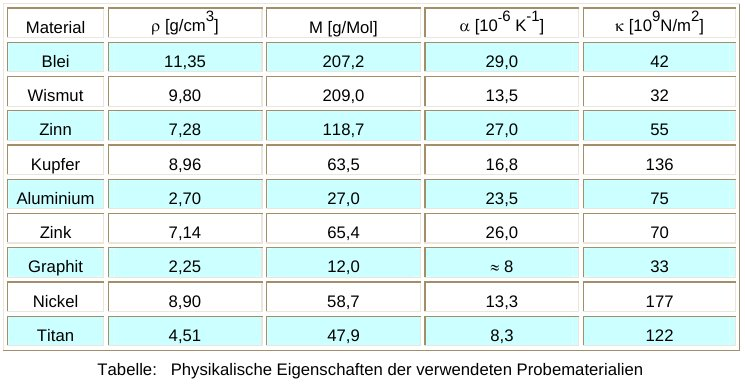
\includegraphics[width=0.8\textwidth]{pics/litwerte.jpg}
\caption{Tabelle der Versuchsanleitung entnommen}
\label{pic_const}
\end{figure}


\section{Auswertung}
\subsection{Wärmekapazität des Kalorimeters}
\label{sec_kalorimeter}
Zu Beginn wird die Wärmekapazität des Kalorimeters $c_g m_g$ ermittelt. In Tabelle \ref{tab_cgmg} sind die Messreihen aufgeführt und der
Wert für die Wärmekapazität aus Gleichung \eqref{eq_cgmg} errechnet. Mit Gleichung \eqref{eq_temp} werden im Zuge der restlichen 
Auswertung die gemessenen Thermospannungen in Temperaturen umgerechnet. Masse $m_y$ und $m_x$ werden in Durchführung auf gleichen Wert
gebracht. Die spezifische Wärmekapazität von Wasser wird zu $c_w$ = 4,18 J/gK angegeben.
\begin{table}[H]
 \begin{tabular}{c|c|c|c|c|c|c|c}
 $U_x$ in V & $T_x$ in $^\circ$C & $U_y$ in V & $T_y$ in $^\circ$C & $U_m$ in V & $T_m$ in $^\circ$C & $m_{x,y}$ in g & $c_g m_g$ in J/K\\
 \hline
0,74&	18,5&	3,66&	89,5&	2,00&	49,6&	300&	360,89\\
0,87&	21,7&	4,08&	99,5&	2,24&	55,4&	300&	388,39\\
 \end{tabular}
\caption{Wärmekapazität des Kalorimeters}
\label{tab_cgmg}
\end{table}
Somit ergibt sich die Wärmekapazität des Kalorimeters ohne Fehlerrechnung zu 
\begin{align}
c_g m_g = 374,64 \, \frac{\text{J}}{\text{K}}.
\end{align}

\subsection[spezifische Wärmekapazität verschiedener Materialien]{spezifische Wärmekapazität bei konstantem Druck von verschiedenen Materialien}
Um annehmbare Werte für den weiteren Verlauf zu erhalten, wird der deutlich zu hohe Wert für die Wärmekapazität des Kalorimeters aus Abschnitt
\ref{sec_kalorimeter} von nun an als 100 J/K angenommen. 

Zur Berechnung der spezifischen Wärmekapazität bei konstantem Druck der untersuchten Materialien wird Gleichung \eqref{eq_ck} unter Verwendung der in Tabelle
\ref{tab_ck} aufgeführten Größen verwandt. Die Masse des Wassers ist hierbei fortwährend $m_w$ = 300 g.

\begin{table}[H]
 \begin{tabular}{l|c|c|c|c|c|c|c}
 Probe ($m_k$)& $U_w$ in V & $T_w$ in $^\circ$C & $U_k$ in V & $T_k$ in $^\circ$C & $U_m$ in V & $T_m$ in $^\circ$C & $c_k$ in J/gK\\
 \hline
Blei&	0,79&	19,8&	3,99&	97,4&	0,86&	21,5 & 0,06\\
526,13 g&	0,73&	18,3&	3,99&	97,4&	0,91&	22,7 & 0,15\\
	&0,84&	21,0&	3,99&	97,4&	0,92&	23,0 & 0,07\\
	\hline
Graphit	&0,84&	21,0&	3,99&	97,4&	0,98&	24,5 & 0,26\\
247,29	g&0,87&	21,7&	3,99&	97,4&	0,98&	24,5 & 0,20\\
	&0,85&	21,2&	3,99&	97,4&	0,98&	24,5 & 0,24\\
	\hline
Aluminium&	0,86&	21,5&	3,99&	97,4&	0,98&	24,5 & 0,22\\
253,10 g	& & & & & & &				\\ \hline

 \end{tabular}
\caption{spezifische Wärmekapazität verschiedener Proben}
\label{tab_ck}
\end{table}

\subsection{Atomwärme bei konstantem Volumen}
\label{sec_atomwaerme}
Die gesuchte Atomwärme bei konstantem Druck $C_P$ lässt sich aus folgender Beziehung bestimmen
\begin{align}
 C_P = c_k \cdot M_{mol}.
\end{align}
Mit den Konstanten aus Abbildung \ref{pic_const} ergeben sich die Werte in Tabelle \ref{tab_cp}.
\begin{table}[H]
 \begin{tabular}{l|c}
 Probe & $C_P$ in J/MolK\\
 \hline
Blei &19,47\\
Graphit &2,83\\
Aluminium &5,90
 \end{tabular}
\caption{Atomwärme bei konstantem Druck der untersuchten Proben}
\label{tab_cp}
\end{table}
Mit den erlangten Werten lässt sich nun die Atomwärme bei konstantem Volumen aus der Relation \eqref{eq_molwaerme} errechnen 
(siehe Tabelle \ref{tab_cv}), die für den Vergleich zum Dulong-Petitschen Gesetz nötig ist. Die benötigten Konstanten sind ebenfalls 
Abbildung \ref{pic_const} entnehmen.
\begin{table}[H]
 \begin{tabular}{l|c}
 Probe & $C_V$ in J/MolK\\
 \hline
Blei &17,76\\
Graphit &2,80\\
Aluminium &5,93
\end{tabular}
\caption{Atomwärme bei konstantem Volumen der untersuchten Proben}
\label{tab_cv}
\end{table}

\section{Diskussion}
Der Wert für die Molwärme aus dem Dulong-Petitschen Gesetz beträgt

\begin{align}
 C_V = 3R = 24,94  \, \frac{\text{J}}{\text{K}}.
\end{align}

Für die experimentelle Bestimmung eben jener ist letztlich die Ermittlung der spezifischen Wärmekapazität entscheidend. In Tabelle 
\ref{tab_diskussion} sind die aus Literaturwerten für die spezifischen Wärmekapazitäten$^{[2]}$ die theoretischen Molwärmewerte, sowie
jene in Abschnitt \ref{sec_atomwaerme} errechneten Werte und die Abweichung zum Dulong-Petit Gesetz aufgeführt.
\begin{table}[H]
 \begin{tabular}{l|c|c|c}
 Probe & $C_{theo}$ in J/K	& $C_{exp}$ in J/K & $\Delta C_{exp,DP}$ in J/K\\
 \hline
Blei	&25,01	&17,76	&29\% \\
Graphit	&8,55	&2,80	&89\% \\
Aluminium	&23,08	&4,92	&80\% 
 \end{tabular}
\caption{Theoretische Werte und Vergleich experimenteller Werten zum Dulong-Petit}
\label{tab_diskussion}
\end{table}

Es lässt sich unschwer erkennen, dass die experimentellen Werte allesamt deutlich unter den theoretischen Erwartungen liegen. Der 
experimentell bestimmte $c_gm_g$-Wert von 374,64 J/K hätte aufgrund der linearen Abhängigkeit zwischen ihm und der spezifischen 
Wärmekapazität höhere Molwärmewerte ergeben. Jedoch gilt die Wärmekapazität für das Kalorimeter als 100 J/K als gegeben. Im Falle
für Aluminium lässt sich das darauf zurückführen, dass lediglich eine Messreihe besteht und diese wohl starken Messfehlern unterliegt,
wie die zu kurze Abwartezeit für die Einstellung einer Ausgleichstemperatur. Die Werte für Blei zeigen als einzige eine etwaige 
Übereinstimmung.

Aus den aufgeführten Werten kann man erkennen, dass Blei und Aluminium dem Dulong-Petitschen Gesetz folgen. Das liegt an den hohen Massen
der Stoffe. Daher fällt Graphit, als recht leichtes Material auch hinaus.

\parskip 340pt
\Large{Literatur}\\\\
\large{[1] Versuchsanleitung - Das Dulong-Petitsche Gesetz}\\\\
\large{[2] Hoppe A., \textit{Periodensystem der Elemente}, URL: \href{http://www.periodensystem.info}{http://www.periodensystem.info}}\\\\

% ========================================
%	Literaturverzeichnis
% ========================================

%\bibliographystyle{plainnat}			% Bibliographie-Style auswählen
%\bibliography{BIBDATEI}			% Literaturverzeichnis

% ========================================
%	Das Dokument endent
% ========================================

\end{document}
